%% abtex2-modelo-relatorio-tecnico.tex, v<VERSION> laurocesar
%% Copyright 2012-<COPYRIGHT_YEAR> by abnTeX2 group at http://www.abntex.net.br/
%%
%% This work may be distributed and/or modified under the
%% conditions of the LaTeX Project Public License, either version 1.3
%% of this license or (at your option) any later version.
%% The latest version of this license is in
%%   http://www.latex-project.org/lppl.txt
%% and version 1.3 or later is part of all distributions of LaTeX
%% version 2005/12/01 or later.
%%
%% This work has the LPPL maintenance status `maintained'.
%%
%% The Current Maintainer of this work is the abnTeX2 team, led
%% by Lauro César Araujo. Further information are available on
%% http://www.abntex.net.br/
%%
%% This work consists of the files abntex2-modelo-relatorio-tecnico.tex,
%% abntex2-modelo-include-comandos and abntex2-modelo-references.bib
%%

% ------------------------------------------------------------------------
% ------------------------------------------------------------------------
% abnTeX2: Modelo de Relatório Técnico/Acadêmico em conformidade com
% ABNT NBR 10719:2015 Informação e documentação - Relatório técnico e/ou
% científico - Apresentação
% ------------------------------------------------------------------------
% ------------------------------------------------------------------------

\documentclass[
	% -- opções da classe memoir --
	12pt,				% tamanho da fonte
	%openright,			% capítulos começam em pág ímpar (insere página vazia caso preciso)
	oneside,			% twoside para impressão em recto e verso. Oposto a oneside
	a4paper,			% tamanho do papel.
	% -- opções da classe abntex2 --
	%chapter=TITLE,		% títulos de capítulos convertidos em letras maiúsculas
	%section=TITLE,		% títulos de seções convertidos em letras maiúsculas
	%subsection=TITLE,	% títulos de subseções convertidos em letras maiúsculas
	%subsubsection=TITLE,% títulos de subsubseções convertidos em letras maiúsculas
	% -- opções do pacote babel --
	english,			% idioma adicional para hifenização
	brazil,				% o último idioma é o principal do documento
	]{abntex2}


% ---
% PACOTES
% ---

% ---
% Pacotes fundamentais
% ---
\usepackage{lmodern}			% Usa a fonte Latin Modern
\usepackage[T1]{fontenc}		% Selecao de codigos de fonte.
\usepackage[utf8]{inputenc}		% Codificacao do documento (conversão automática dos acentos)
\usepackage{indentfirst}		% Indenta o primeiro parágrafo de cada seção.
\usepackage{color}				% Controle das cores
\usepackage{graphicx}			% Inclusão de gráficos
\usepackage{microtype} 			% para melhorias de justificação
% ---

% ---
% Pacotes adicionais, usados no anexo do modelo de folha de identificação
% ---
\usepackage{multicol}
\usepackage{multirow}
% ---

% ---
% Pacotes adicionais, usados apenas no âmbito do Modelo Canônico do abnteX2
% ---
\usepackage{lipsum}				% para geração de dummy text
% ---

% ---
% Pacotes de citações
% ---
\usepackage[brazilian,hyperpageref]{backref}	 % Paginas com as citações na bibl
\usepackage[alf]{abntex2cite}	% Citações padrão ABNT

% ---
% Pacote de gráficos
% ---
% \usepackage{tikz}

% ---
% Pacote para adicionar facilmente quebra de linha em células das tabelas
% ---
\usepackage{makecell}

% ---
% Pacote para melhorar a aparência das tabelas e permitir formatação complexa
% ---
\usepackage{booktabs}

% ---
% Pacote para permitir tabelas ocuparem múltiplas páginas (cuidado com Overleaf gratuito)
% ---
\usepackage{longtable}

% ---
% Pacote para controlar formatação das legendas
% ---
\usepackage{caption}
\captionsetup[longtable]{font=normalsize,singlelinecheck=false,justification=raggedright,position=top}

% ---
% Pacote para manter as tabelas dentro das seções em que foram criadas
% ---
\usepackage[section]{placeins}

% ---
% Pacote para controlar floats, não usar em conjunto com o pacote float comum
% ---
% \usepackage{floatrow}
% \floatsetup[longtable]{LTcapwidth=table}

% ---
% CONFIGURAÇÕES DE PACOTES
% ---

% ---
% Configurações do pacote backref
% Usado sem a opção hyperpageref de backref
\renewcommand{\backrefpagesname}{Citado na(s) página(s):~}
% Texto padrão antes do número das páginas
\renewcommand{\backref}{}
% Define os textos da citação
\renewcommand*{\backrefalt}[4]{
	\ifcase #1 %
		Nenhuma citação no texto.%
	\or
		Citado na página #2.%
	\else
		Citado #1 vezes nas páginas #2.%
	\fi}%
% ---

% ---
% Configurações do pacote tikz
% ---
% \usetikzlibrary{shapes.geometric, arrows.meta, positioning}

% ---
% Informações de dados para CAPA e FOLHA DE ROSTO
% ---
\titulo{NotoriousNote \\ \huge{Visão do Projeto} \\ \Large{Abordagem Tradicional}}
\autor{Equipe EmptyCoffeeCups \\ Davi Antônio da Silva Santos \and Marcos Adriano \and Jonathan Jorge Barbosa Oliveira \and Wellington Jonathan}
\local{Brasília, Distrito Federal, Brasil}
\data{2021, 2021.05.11-preview}
\instituicao{%
  Universidade de Brasília -- UnB
  \par
  Faculdade do Gama -- FGA
}
\tipotrabalho{Relatório técnico}
% O preambulo deve conter o tipo do trabalho, o objetivo,
% o nome da instituição e a área de concentração
\preambulo{Documento de visão e planejamento do projeto NotoriousNote.}
% ---

% ---
% Configurações de aparência do PDF final

% alterando o aspecto da cor azul
\definecolor{blue}{RGB}{41,5,195}

% informações do PDF
\makeatletter
\hypersetup{
     	%pagebackref=true,
		pdftitle={\@title},
		pdfauthor={\@author},
    	pdfsubject={\imprimirpreambulo},
	    pdfcreator={LaTeX with abnTeX2},
		pdfkeywords={abnt}{latex}{abntex}{abntex2}{relatório técnico},
		colorlinks=true,       		% false: boxed links; true: colored links
    	linkcolor=blue,          	% color of internal links
    	citecolor=blue,        		% color of links to bibliography
    	filecolor=magenta,      		% color of file links
		urlcolor=blue,
		bookmarksdepth=4
}
\makeatother
% ---

% ---
% Espaçamentos entre linhas e parágrafos
% ---

% O tamanho do parágrafo é dado por:
\setlength{\parindent}{1.3cm}

% Controle do espaçamento entre um parágrafo e outro:
\setlength{\parskip}{0.2cm}  % tente também \onelineskip

% ---
% compila o indice
% ---
\makeindex
% ---

% ----
% Início do documento
% ----
\begin{document}

% Seleciona o idioma do documento (conforme pacotes do babel)
%\selectlanguage{english}
\selectlanguage{brazil}

% Retira espaço extra obsoleto entre as frases.
\frenchspacing

% ----------------------------------------------------------
% ELEMENTOS PRÉ-TEXTUAIS
% ----------------------------------------------------------
% \pretextual

% ---
% Capa
% ---
\imprimircapa
% ---

% ---
% Folha de rosto
% (o * indica que haverá a ficha bibliográfica)
% ---
\imprimirfolhaderosto*
% ---

% ---
% Anverso da folha de rosto:
% ---

% {
% \ABNTEXchapterfont

% \vspace*{\fill}

% Conforme a ABNT NBR 10719:2015, seção 4.2.1.1.1, o anverso da folha de rosto
% deve conter:

% \begin{alineas}
%   \item nome do órgão ou entidade responsável que solicitou ou gerou o
%   relatório;
%   \item título do projeto, programa ou plano que o relatório está relacionado;
%   \item título do relatório;
%   \item subtítulo, se houver, deve ser precedido de dois pontos, evidenciando a
%   sua subordinação ao título. O relatório em vários volumes deve ter um título
%   geral. Além deste, cada volume pode ter um título específico;
%   \item número do volume, se houver mais de um, deve constar em cada folha de
%   rosto a especificação do respectivo volume, em algarismo arábico;
%   \item código de identificação, se houver, recomenda-se que seja formado
%   pela sigla da instituição, indicação da categoria do relatório, data,
%   indicação do assunto e número sequencial do relatório na série;
%   \item classificação de segurança. Todos os órgãos, privados ou públicos, que
%   desenvolvam pesquisa de interesse nacional de conteúdo sigiloso, devem
%     informar a classificação adequada, conforme a legislação em vigor;
%   \item nome do autor ou autor-entidade. O título e a qualificação ou a função
%   do autor podem ser incluídos, pois servem para indicar sua autoridade no
%   assunto. Caso a instituição que solicitou o relatório seja a mesma que o
%   gerou, suprime-se o nome da instituição no campo de autoria;
%   \item local (cidade) da instituição responsável e/ou solicitante; NOTA: No
%   caso de cidades homônimas, recomenda-se o acréscimo da sigla da unidade da
%   federação.
%   \item ano de publicação, de acordo com o calendário universal (gregoriano),
%   deve ser apresentado em algarismos arábicos.
% \end{alineas}

% \vspace*{\fill}
% }

% ---
% Agradecimentos
% ---
% \begin{agradecimentos}
% O agradecimento principal é direcionado a Youssef Cherem, autor do
% \nameref{formulado-identificacao} (\autopageref{formulado-identificacao}).

% Os agradecimentos especiais são direcionados ao Centro de Pesquisa em
% Arquitetura da Informação\footnote{\url{http://www.cpai.unb.br/}} da Universidade de
% Brasília (CPAI), ao grupo de usuários
% \emph{latex-br}\footnote{\url{http://groups.google.com/group/latex-br}} e aos
% novos voluntários do grupo
% \emph{\abnTeX}\footnote{\url{http://groups.google.com/group/abntex2} e
% \url{http://www.abntex.net.br/}}~que contribuíram e que ainda
% contribuirão para a evolução do abn\TeX.

% \end{agradecimentos}
% ---

% ---
% RESUMO
% ---

% resumo na língua vernácula (obrigatório)
% \setlength{\absparsep}{18pt} % ajusta o espaçamento dos parágrafos do resumo
% \begin{resumo}
%  Segundo a \citeonline[3.1-3.2]{NBR6028:2003}, o resumo deve ressaltar o
%  objetivo, o método, os resultados e as conclusões do documento. A ordem e a extensão
%  destes itens dependem do tipo de resumo (informativo ou indicativo) e do
%  tratamento que cada item recebe no documento original. O resumo deve ser
%  precedido da referência do documento, com exceção do resumo inserido no
%  próprio documento. (\ldots) As palavras-chave devem figurar logo abaixo do
%  resumo, antecedidas da expressão Palavras-chave:, separadas entre si por
%  ponto e finalizadas também por ponto.

%  \noindent
%  \textbf{Palavras-chaves}: latex. abntex. editoração de texto.
% \end{resumo}
% ---

% Histórico de revisão
\chapter*[Histórico de Revisões]{Histórico de Revisões}

\IBGEtabfontsize
\begin{longtable}{@{}p{0.1\textwidth}p{0.1\textwidth}p{0.6\textwidth}p{0.1\textwidth}@{}}
%\caption{}
%\label{} \\
\toprule
\textbf{Data} & \textbf{Versão} & \textbf{Descrição} & \textbf{Autor} \\ \midrule \endhead
10/05/2021 & 2021.05.10-preview & \begin{tabular}{@{}p{0.6\textwidth}@{}}Versão inicial deste documento de visão por abordagem tradicional produzida a partir da versão 2021.05.04-preview do documento de visão por abordagem ágil \\ Remoção da parte de abordagem ágil \\ Renomear parte Abordagem Tradicional para Atividades da Engenharia de Requisitos \\ Renomear capítulo Requisitos Tradicionais para Requisitos \\ Alterar descrição do RF19 \\ Corrigir tabela de planejamento de gerência para refletir a mudança de paradigma da Engenharia de Requisitos \\ Atualizar Android Studio de 4.1.3 para 4.2 \\ Atualizar Flutter de 2.0.4 para 2.0.6 \\ Atualizar Kotlin para 1.5.0 \\ Especificar a diferença entre o Gradle e o Gradle Plug-in \\ Atualizar extensão Kotlin da versão 1.4.31-release-Studio4.1 para 202-1.5.0-release-764-AS8194.7 \\ Atualizar plug-in Dart de 201.9335 para 202.8488 \\ Atualizar plug-in Flutter de 55.1.1 para 56.0.2 \end{tabular} & Davi Antônio da Silva Santos \\ \midrule
11/05/2021 & 2021.05.11-preview & \begin{tabular}{@{}p{0.6\textwidth}@{}}Adicionar risco RS07 \\ Iniciar capítulo de lições aprendidas \\ Atualizar MVP \\ Modificar as descrições dos requisitos funcionais \\ Modificar nomes dos casos de uso para que estejam adequados ao padrão (verbo de ação) \\ Atualizar diagrama de casos de uso corrigindo nomes e relações de extensão \\ Alteração do Processo de Desenvolvimento e Mensuração, da Matriz de comunicação, dos Critérios de Replanejamento e da Organização do projeto para refletir a perspectiva tradicional \\ Especificação do UC01 \\ Acrescentar necessidades à tabela de requisitos funcionais \\ Adicionar informações relativas ao MVP, à implementação na etapa ágil e reformatar tabela de relação entre requisitos e casos de uso \end{tabular} & Equipe EmptyCoffeCups \\ \midrule
 & & & \\ \bottomrule
\end{longtable}
\cleardoublepage

% ---
% inserir lista de ilustrações
% ---
\pdfbookmark[0]{\listfigurename}{lof}
\listoffigures*
\cleardoublepage
% ---

% ---
% inserir lista de tabelas
% ---
\pdfbookmark[0]{\listtablename}{lot}
\listoftables*
\cleardoublepage
% ---

% ---
% inserir lista de abreviaturas e siglas
% ---
\begin{siglas}
  \item[API] \foreignlanguage{english}{\textit{Application Programming Interface}}
  \item[BD] Banco de Dados
  \item[BLoC] \foreignlanguage{english}{\textit{Business Logic of Component}}
  \item[DB] \foreignlanguage{english}{\textit{Database}}
  \item[IDE] \foreignlanguage{english}{\textit{Integrated Development Environment}}
  \item[SAFe] \foreignlanguage{english}{\textit{Scaled Agile Framework}}
  \item[SDK] \foreignlanguage{english}{\textit{Software Development Kit}}
  \item[SOLID] \foreignlanguage{english}{\textit{Single responsibility, Open-closed, Liskov substitution, Interface segregation, Dependency inversion}}
  \item[UI] \foreignlanguage{english}{\textit{User Interface}}
  \item[UnB] Universidade de Brasília
\end{siglas}
% ---

% ---
% inserir lista de símbolos
% ---
% \begin{simbolos}
%   \item[$ \Gamma $] Letra grega Gama
%   \item[$ \Lambda $] Lambda
%   \item[$ \zeta $] Letra grega minúscula zeta
%   \item[$ \in $] Pertence
% \end{simbolos}
% ---

% ---
% inserir o sumario
% ---
\pdfbookmark[0]{\contentsname}{toc}
\tableofcontents*
\cleardoublepage
% ---


% ----------------------------------------------------------
% ELEMENTOS TEXTUAIS
% ----------------------------------------------------------
\textual
%[Este artefato deve ser utilizado como guia para o registro das informações gerais do projeto. Deve ser refinado e atualizado ao longo do projeto].

\chapter{Introdução}
%\section{Problema}

\section{Declaração do Problema}
%[Forneça uma declaração resumindo o problema que está sendo resolvido por este projeto. O seguinte formato pode ser usado:]

\begin{table}[ht]
\IBGEtab{%
\caption{Declaração do problema}%
\label{tab:declaracao_problema}%
}{%
\begin{tabular}{@{}p{0.29\textwidth}p{0.7\textwidth}@{}}
\toprule
% descreva o problema
O problema & grande quantidade de atividades simultâneas exigidas pela sociedade atual \\ \midrule
% informe as partes interessadas afetadas pelo problema
Afeta & pessoas que possuem dificuldade em organizar seus compromissos caso não os anotem \\ \midrule
% qual é o impacto desse problema?
Cujo impacto é & risco de não cumprimento de compromissos e desorganização das tarefas individuais \\ \midrule
% liste alguns benefícios principais de uma solução de sucesso
Uma solução de sucesso seria & permitir que os criem anotações com a possibilidade de configurar lembretes para notificar anotações específicas, criem anotações para lista de tarefas, classifiquem anotações por grupos, realizem backups remotos e locais das anotações \\ \bottomrule
\end{tabular}%
}{%\fonte{}%
}
\end{table}

\section{Objetivos do Projeto}
%[Forneça o objetivo principal do projeto, e objetivos secundários (caso haja)]
\subsection{Objetivos primários}
Criar uma aplicação que permita o usuário crie anotações, listas de tarefa, lembretes para as anotações. Também deve ser possível ao usuário acessar \textit{templates} de anotações para criar modelos comuns mais rapidamente.

\subsection{Objetivos secundários}
A aplicação também deve ser capaz de exportar os dados de suas notas e listas de tarefas para formatos que podem ser importados em outros aplicativos ou armazenados em dispositivos externos: JSON, \texttt{org-mode} e texto puro. Além disso, também deve ser possível fazer o backup dos dados do dispositivo na nuvem e compartilhar a informação com outros aplicativos usando funções nativas do sistema operacional móvel.

\chapter{\foreignlanguage{english}{\textit{Stakeholders}}}
% [Forneça a lista de stakeholders envolvidos no projeto]

\begin{table}[ht]
\IBGEtab{%
\caption{Lista das partes interessadas (\textit{stakeholders}) envolvidas no projeto}%
\label{tab:stakeholders}%
}{%
\begin{tabular}{@{}p{0.2\textwidth}p{0.25\textwidth}p{0.5\textwidth}@{}}
\toprule
\textbf{Nome} & \textbf{Descrição} & \textbf{Responsabilidades} \\ \midrule
% Nomeie o tipo de parte interessada & Descreva resumidamente a parte interessada & Resuma as principais responsabilidades das partes interessadas com relação ao sistema que está sendo desenvolvido; \\ ou seja, seu interesse como parte interessada. Por exemplo, esta parte interessada:\\ garante que o sistema será sustentável\\ garante que haverá uma demanda de mercado para as características do produto\\ monitora o progresso do projeto\\ aprova financiamento\\ e assim por diante
Professor orientador & Professor da disciplina de Requisitos de Software & \makecell[c{p{0.5\textwidth}}]{Monitora o progresso do projeto \\ Auxilia na validação e verificação de requisitos} \\ \midrule
Desenvolvedores & Alunos da disciplina de Requisitos de Software & \makecell[c{p{0.5\textwidth}}]{Elicitam, analisam, especificam, validam, verificam e gerenciam requisitos\\ Desenvolvem e testam o software \\ Produzem um software utilizável} \\ \midrule
Usuário & Pessoas que utilizarão o aplicativo & \makecell[c{p{0.5\textwidth}}]{Utilizar a aplicação móvel\\ Reportar problemas aos desenvolvedores} \\ \bottomrule
\end{tabular}%
}{%\fonte{}%
}
\end{table}

\chapter{Visão Geral do Produto}

\section{Declaração de Posição do Produto}
%[Forneça uma declaração geral resumindo, no nível mais alto, a posição exclusiva que o produto pretende preencher no mercado. Uma declaração de posição do produto comunica a intenção da aplicação e a importância do projeto para todo o pessoal envolvido. O seguinte formato pode ser usado:]

\begin{table}[ht]
\IBGEtab{%
\caption{Declaração de posição do produto.}%
\label{tab:declaracao_posicao_prodututo}%
}{%
\begin{tabular}{@{}p{0.2\textwidth}p{0.8\textwidth}@{}}
\toprule
% cliente alvo
\textbf{Para} & usuários de \textit{smartphone} Android \\ \midrule
% declaração da necessidade ou oportunidade
\textbf{Quem} & usuários que queiram controle sobre as suas notas escritas em um celular, mas não querem abandonar a comodidade de armazenarem seus dados na nuvem \\ \midrule
% O [nome do produto] & é um/uma [categoria do produto]
\textbf{O NotoriousNote} & é uma aplicação móvel de registro de notas \\ \midrule
% declaração do principal benefício; ou seja, a razão convincente para comprar, utilizar, etc.
\textbf{Que} & permite que o usuário exporte os dados da própria aplicação, de modo que possa armazená-los em outro lugar com o objetivo de, por exemplo, realizar backup de notas importantes \\ \hline
% alternativa competitiva primária
\textbf{Ao contrário} & do Google Keep, que dificulta a exportação das notas e listas de tarefas feitas no próprio aplicativo \\ \midrule
% declaração de diferenciação primária
\textbf{Nosso produto} & permite que o usuário exporte os seus dados em um formato legíveis (JSON, texto puro e \texttt{org-mode}) que podem ser usado em outras aplicações \\ \bottomrule
\end{tabular}%
}{%\fonte{}%
}
\end{table}

\section{Mínimo Produto Viável (MVP)}
%[Forneça uma lista de características mínimas que o produto deve possuir para que possa ser lançado]
O mínimo produto viável (MVP) deve possuir as seguintes características funcionais:
\begin{itemize}
    \item Criar, apagar, editar e visualizar de notas de texto com título e conteúdo;
    \item Criar, apagar, editar e visualizar etiquetas;
    \item Atribuir etiquetas a uma anotação.
    % \item Exportar notas e listas de tarefas em texto puro;
    % \item Visualizar notas por etiquetas específicas.
    % \item Criação de listas de tarefa com título e tarefas que podem ser registradas como terminadas ou não;
    % \item Capacidade de salvar notas e listas de tarefa em nuvem (Cloud Firestore);
    % \item Capacidade de exportar notas e listas de tarefas em JSON;
    % \item Capacidade de ler notas e listas de tarefas salvas localmente em JSON.
\end{itemize}

\chapter{Visão Geral do Projeto}
\section{Organização do Projeto}
%[apresentada a divisão de atribuições e responsabilidades entre os membros do projeto, sem qualquer relação de hierarquia ou grau de importância. Todos os integrantes são igualmente importantes e responsáveis pelo sucesso do projeto.]
% A organização do projeto seguirá a divisão de papéis proposta pelo \textit{framework} Scrum \cite{scrum_guide}.

\begin{table}[ht]
\IBGEtab{%
\caption{Organização do projeto}%
\label{tab:organizacao_projeto}%
}{%
\begin{tabular}{@{}p{0.2\textwidth}p{0.24\textwidth}p{0.24\textwidth}p{0.24\textwidth}@{}}
\toprule
\textbf{Papel} & \textbf{Atribuições} & \textbf{Responsável} & \textbf{Participantes} \\ \midrule
\textit{Developer} & \makecell[c{p{0.24\textwidth}}]{Membro da equipe \\ Escrita e construção do software} & Jonathan Jorge, \foreignlanguage{english}{Wellington} Jonathan & Davi Antônio, Jonathan Jorge, Marcos Adriano, Wellington Jonathan\\ \midrule
\textit{Process Engineer} & Desenvolve, adapta e oferece suporte aos materiais de processo de software do projeto & Marcos Adriano & - \\ \midrule
\textit{Project Manager} & Responsável por manter o conceito das funcionalidades e melhorias, de forma que sigam a visão definida para o produto ou projeto. & Davi Antônio & - \\ \midrule
\textit{Configuration Manager} & Mantém infraestrutura e ambiente de desenvolvimento & Davi Antônio & - \\ \midrule
Professor Orientador & Professor da disciplina de Requisitos de Software & Professor Dr. Marsicano & Professor Dr. Marsicano \\ \bottomrule
\end{tabular}%
}{%\fonte{}%
}
\end{table}

\chapter{Ferramentas, Ambiente e Infraestrutura}
\section{Hardware}
% [Esta seção apresenta a infra-estrutura de hardware adequada para o desenvolvimento do projeto.]
% [Exemplo:

\begin{table}[ht]
\IBGEtab{%
\caption{Infraestrutura de hardware necessária}%
\label{tab:infra_hardware}%
}{%
\begin{tabular}{@{}p{0.14\textwidth}p{0.14\textwidth}p{0.27\textwidth}p{0.05\textwidth}p{0.2\textwidth}@{}}
\toprule
\textbf{Perfil} & \textbf{Tipo} & \textbf{Configurações} & \textbf{Qtd.} & \textbf{Observação} \\ \midrule
Desenvolvedor & Computador & \makecell[c{p{0.27\textwidth}}]{Interface USB \\ Mínimo 8 GiB RAM \\ Resolução de tela mínima 1280x800 px.} & 04 & - \\ \bottomrule
\end{tabular}%
}{%\fonte{}%
}
\end{table}
\newpage%
\section{Software}
%[Esta seção apresenta a infra-estrutura de software adequada para o desenvolvimento do projeto.]
%[Exemplo:
\begin{table}[ht]
\caption{Infraestrutura de software necessária}%
\label{tab:ambiente_software}
\centering
\IBGEtabfontsize
\begin{tabular}{@{}p{0.125\textwidth}p{0.145\textwidth}p{0.145\textwidth}p{0.135\textwidth}p{0.100\textwidth}p{0.115\textwidth}@{}}
\toprule
\textbf{Perfil} & \textbf{Tipo} & \textbf{Nome} & \textbf{Versão} & \textbf{Licenças}  & \textbf{Observação} \\ \midrule
Todos & Controle de Versão & Git & 2.25.1 ou superior & 04  & - \\ \midrule
Todos & IDE & Android Studio & 4.2 & 04  & - \\ \midrule
Todos & SDK & Flutter & 2.0.6 & 04  & - \\ \midrule
Todos & Linguagem de programação & Dart & 2.12.3 & 04  & - \\ \midrule
Todos & Linguagem de programação & Kotlin & 1.5.0 & 04  & - \\ \midrule
Todos & Extensão do Android Studio & Dart & 202.8488 & 04  & - \\ \midrule
Todos & Extensão do Android Studio & Flutter & 56.0.2 & 04  & - \\ \midrule
Todos & Extensão do Android Studio & Kotlin & 202-1.5.0-release-764-AS8194.7 & 04  & - \\ \midrule
Todos & Pacote Flutter & provider & \^{}5.0.0 & 04 & - \\ \midrule
Todos & Pacote Flutter & sqflite & \^{}2.0.0+3 & 04 & - \\ \midrule
Todos & Pacote Flutter & firebase\_core & \^{}1.0.2 & 04 & - \\ \midrule
Todos & Pacote Flutter & firebase\_auth & \^{}1.0.1 & 04  & - \\ \midrule
Todos & Pacote Flutter & cloud\_firestore & \^{}1.0.3 & 04  & - \\ \midrule
Todos & Dependência Android & google-services & 4.3.5 & 04  & - \\ \midrule
Todos & Dependência Android & firebase-bom & 26.8.0 & 04  & - \\ \midrule
Todos & Ferramenta de compilação & gradle-plug-in & 4.2 & 04  & - \\ \midrule
Todos & Ferramenta de compilação & gradle & 6.9 & 04  & - \\ \midrule
Todos & Ferramenta de compilação & Android SDK Build Tools & 30.0.3 & 04  & - \\ \bottomrule
\end{tabular}%
\end{table}

\chapter{Processo de Gerência de Projeto}
\section{Planejamento das Fases e Iterações do Projeto}
% [Registrar o projeto, as fases de seu ciclo de vida e suas iterações, especificando suas datas de início e de fim, bem como os produtos a serem gerados.]

\begin{table}[ht]
\IBGEtab{%
\caption{Planejamento de gerência de projeto}%
\label{tab:fases_iteracoes}%
}{% p{0.14\textwidth} %\makecell[c{p{0.27\textwidth}}]{}
\begin{tabular}{@{}lllp{0.7\textwidth}@{}}
\toprule
\textbf{Iteração} & \textbf{Início} & \textbf{Fim} & \textbf{Incrementos Esperados} \\ \midrule
1 & 06/04 & 22/04 & \begin{tabular}{@{}p{0.7\textwidth}@{}}Levantar problemas, necessidades, requisitos \\ Organizar requisitos em casos de uso \\ Elaborar diagrama de casos de uso \\ Atualização do documento de visão (ainda misturando abordagem ágil e tradicional) com necessidades, requisitos, casos de uso e diagrama de casos de uso\end{tabular} \\ \midrule
2 & 27/04 & 13/05 & \begin{tabular}{@{}p{0.7\textwidth}@{}}Separar documentos de visão em ágil e tradicional \\ Especificar casos de uso do MVP \\ Separar repositórios em código desenvolvido com as histórias e com os casos de uso \\ Geração da APK otimizada para lançamento \\ Entrega da versão final do documento de visão tradicional\end{tabular} \\ \bottomrule
\end{tabular}%
}{%\fonte{}%
}
\end{table}

\section{Processo de Desenvolvimento e Mensuração}
% [Especifique como será acompanhado o progresso, por exemplo, por meio de reuniões de revisão diárias, avaliações de iteração, relatórios de Burndown de Projeto e Burndown de Iteração.]
A equipe utilizará um processo de desenvolvimento tradicional semelhante ao Processo Unificado, mas bastante simplificada. A plataforma Github servirá como repositório remoto para o sistema de versionamento distribuído Git, que será utilizado para o controle de versão do código fonte e do documento de visão.

O documento de visão será elaborado em comum acordo entre os membros da equipe e conterá as especificações do MVP, do ambiente de desenvolvimento, os problemas do cliente, necessidades, requisitos funcionais e os casos de uso derivados. Esse documento também manterá um histórico de modificações e das ações tomadas em cada uma das iterações.

Os requisitos serão derivados a partir das necessidades do usuário levantadas pela equipe, derivadas a partir dos problemas encontrados. Os requisitos serão organizados em casos de uso e somente aqueles que fazem parte do MVP, ou seja, os que trazem maior valor para o cliente, serão especificados e implementados.

% \section{\foreignlanguage{english}{\textit{Milestones}} e Objetivos do Projeto}

\section{Matriz de Comunicação}
A comunicação do grupo é feita principalmente pelo Telegram e por reuniões no Microsoft Teams.
%[Esta seção descreve a estratégia de comunicação adotada para monitoramento do progresso do projeto. Identificar a periodicidade de reuniões e o envio dos relatórios exigidos pelo processo e opcionalmente outros relatórios exigidos pelo cliente.]

\begin{table}[ht]
\IBGEtab{%
\caption{Matriz de comunicação}%
\label{tab:matriz_comunicacao}%
}{%
\begin{tabular}{@{}p{0.25\textwidth}p{0.25\textwidth}p{0.2\textwidth}p{0.25\textwidth}@{}}
\toprule
\textbf{Descrição} & \textbf{Área/Envolvidos} & \textbf{Periodicidade} & \textbf{Produtos Gerados} \\ \midrule
% \multirow{2}{=}{\begin{tabular}[c]{@{}p{0.25\textwidth}@{}}- Acompanhamento das Atividades em Andamento\\ - Acompanhamento dos Riscos, Compromissos, Ações Pendentes, Indicadores \end{tabular}} & - Equipe do Projeto & - Semanal & \multirow{2}{=}{\begin{tabular}[c]{@{}p{0.2\textwidth}@{}}- Ata de reunião\\ - Relatório de situação do projeto \end{tabular}} \\ \cmidrule(lr){2-3}
%  &  & - Quinzenal &  \\ & & & \\ & & & \\ & & & \\ & & & \\ \midrule

- Comunicar situação do projeto & \begin{tabular}[c]{@{}l@{}}- Equipe \\ - Professor\end{tabular} & - No final de cada iteração & \begin{tabular}[c]{@{}p{0.25\textwidth}@{}}- Comunicação com o Professor Orientador\\- Atualizações no documento de visão \end{tabular} \\ \midrule

- Comunicar situação do projeto entre membros & \begin{tabular}[c]{@{}l@{}}- Equipe \\ \end{tabular} & - Semanalmente & \begin{tabular}[c]{@{}p{0.25\textwidth}@{}}- \\  \end{tabular} \\ \midrule

\end{tabular}%
}{%\fonte{}%
}
\end{table}

\section{Escalabilidade do Projeto}

Com o andamento do projeto, previsivelmente ocorreram conflitos que devem ser identificados o mais breve possível, e que devem ser imediatamente solucionados. O tratamento desses conflitos deve ser algo orgânico do fluxo de desenvolvimento de software, e ter antecipadamente para diferentes problemas subsequentes frentes de resolução, sendo que nem todo conflito pode ou deve ser solucionado em uma primeira instancia.

O fluxo do projeto deve ter em seu acompanhamento um monitoramento continuo de revisão e correção. Deve-se garantir quando encontrados conflitos esses devem ser imediatamente tratados com prioridade para o \textit{Project Manager} e escalonados, caso seja necessário, ao Professor Orientador para sua dada resolução, evitando o comprometimento do fluxo de projeto.


\section{Gerenciamento de Riscos}
O objetivo principal da Gestão de Riscos é controlar  impedimentos de qualquer tipo, que possa surgir durante o ciclo de desenvolvimento , impedindo o progresso do projeto de acordo com as previsões iniciais. Dessas forma os riscos elicitados foram os seguintes:
\begin{table}[ht]
\IBGEtab{%
\caption{Lista de riscos}%
\label{tab:lista_riscos}%
}{%
\begin{tabular}{@{}p{0.24\textwidth}p{0.24\textwidth}p{0.24\textwidth}p{0.2\textwidth}@{}}
\toprule
\textbf{Código} & \textbf{Risco} & \textbf{Ação} & \textbf{Nível de Risco} \\ \midrule
RS01 & Não Versionamento do código & Refatoração do código para ser aceito na versão mais recente do projeto. & Médio \\ \midrule
RS02 & Equipe desorganizada & Reunião para alinhar a equipe. & Baixo \\ \midrule
RS03 & Não priorização dos requisitos & Analisar as dependências dos requisitos e priorizar os que há menos dependência & Baixo\\ \midrule
RS04 & Má elicitação dos requisitos (Necessidades, requisitos e casos de uso) & Refazer o requisito e todas as partes que o mesmo está envolvido. & Alto \\ \midrule
RS05 & Falta de comunicação da equipe & Reunir para alinhar a equipe & Médio. \\ \midrule
RS06 & Não integração do código & Refatoração do código para permitir integração & Médio. \\ \midrule
RS07 & Perda de integrante da equipe & Redistribuição das atividades entre os integrantes da equipe & Alto \\ \midrule

\end{tabular}%
}{%\fonte{}%
}
\end{table}
%[Para o Gerenciamento de Riscos devem ser realizadas tarefas, como:
%\begin{itemize}
%\item
 %   \item Identificar todos os riscos possíveis e detectáveis em cada fase do projeto;
 %   \item Executar as ações para mitigar os riscos que tenham um alto grau de exposição ao risco caso este ocorra na Lista de Riscos do Projeto;
  %  \item Fazer uma revisão da lista dos riscos periodicamente, com o propósito de averiguar uma possível incidência de um risco e ver se há outros riscos ainda não relatados;
   % \item Em caso de confirmação de um risco previsto, agir no sentido de contingenciá-lo conforme programado;%    \item Registrar os riscos no Painel de Controle do Projeto e no Plano do Projeto (Riscos iniciais);]
%\end{itemize}


\section{Critérios de Replanejamento}
%[Descrever os critérios de replanejamento que serão utilizados, caso seja necessário realizá-lo no projeto.]
Será necessário replanejar o projeto caso algumas dessas situações venha acontecer:
\begin{itemize}
    \item Algum integrante ficar impossibilitado de colaborar com o projeto;
    \item Caso a tecnologia escolhida torne-se inadequada ao desenvolvimento do projeto.
    \item Em casos de \textit{feedbacks} do professor orientador.
\end{itemize}

\part{Atividades da Engenharia de Requisitos}

\chapter{Requisitos}
\section{Necessidades}

\IBGEtabfontsize
\begin{longtable}{@{}p{0.05\textwidth}p{0.2\textwidth}p{0.05\textwidth}p{0.2\textwidth}p{0.2\textwidth}p{0.2\textwidth}@{}}
\caption{Necessidades}
\label{tab:necessidades} \\
\toprule
\textbf{Id.} & \textbf{Necessidade} & \textbf{Prioridade} & \textbf{Problema} & \textbf{Solução Atual} & \textbf{Solução Proposta} \\ \midrule
N1 & Gerenciar anotações & Alta & Dificuldade em organizar múltiplos compromissos de forma eficiente & Gerenciamento dos compromissos em blocos adesivos ou agenda física & Digitalização do processo de registro e gestão das anotações \\ \midrule
N2 & Cópia de segurança das anotações & Média & Ter acesso às anotações sempre que precisar, mesmo em caso de roubos e perdas & Não é realizado backup das anotações & Digitalizar as anotações possibilitará a cópia eficiente das anotações \\ \midrule
N3 &Lembrar compromissos & Média & Recordar dos compromissos de forma simples e eficiente & A lembrança dos compromissos é feita analisando a agenda e anotações periodicamente & Elaboração de um sistema que alerta o usuário dos seus lembretes \\ \bottomrule
\end{longtable}

\section{Requisitos funcionais}
\IBGEtabfontsize
\begin{longtable}{@{}lllp{0.60\textwidth}@{}}
\caption{Requisitos funcionais e necessidades}
\label{tab:requisitos} \\
\toprule
\textbf{Id.} & \textbf{Nec.} & \textbf{Nome} & \textbf{Descrição} \\ \midrule
RF01 & N1 & Criar anotação & O sistema deve permitir criar uma anotação \phantomsection \label{RF01} \\ \midrule
RF02 & N1 & Visualizar anotação & O sistema deve permitir a visualização das anotações \phantomsection \label{RF02} \\ \midrule
RF03 & N1 & Modificar anotação & O sistema deve permitir a modificação das anotações \phantomsection \label{RF03}\\ \midrule
RF04 & N1 & Apagar anotação & O sistema deve permitir apagar anotações \phantomsection \label{RF04} \\ \midrule
RF05 & N1 & Criar etiqueta & O sistema deve permitir criar etiquetas com nome \phantomsection \label{RF05} \\ \midrule
RF06 & N1 & Visualizar etiqueta & O sistema deve permitir visualizar etiquetas \phantomsection \label{RF06} \\ \midrule
RF07 & N1 & Modificar etiqueta & O sistema deve permitir a modificação do nome de cada etiqueta\phantomsection \label{RF07} \\ \midrule
RF08 & N1 & Remover etiqueta & O sistema deve permitir a remoção de etiquetas \phantomsection \label{RF08} \\ \midrule
RF09 & N1 & Atribuir etiqueta & O sistema deve permitir a atribuição de etiquetas a anotações \phantomsection \label{RF09} \\ \midrule

RF10 & N2 & Backup em nuvem & O sistema deve permitir backups em nuvem \phantomsection \label{RF10} \\ \midrule
RF11 & N2 & Criar conta & O sistema deve permitir criar conta para backup em nuvem \phantomsection \label{RF11} \\ \midrule
RF12 & N1 & Criar lista & O sistema deve permitir criação de listas de tarefa \phantomsection \label{RF12} \\ \midrule
RF13 & N1 & Visualizar lista & O sistema deve permitir a visualização de listas de tarefa \phantomsection \label{RF13} \\ \midrule
RF14 & N1 & Modificar lista & O sistema deve permitir a modificação das listas de tarefa \phantomsection \label{RF14} \\ \midrule
RF15 & N1 & Apagar lista & O sistema deve permitir apagar listas de tarefa \phantomsection \label{RF15} \\ \midrule
RF16 & N1 & Criar tarefa & O sistema deve permitir a criação de tarefas \phantomsection \label{RF16} \\ \midrule
RF17 & N1 & Visualizar tarefa & O sistema deve permitir a visualização das tarefas \phantomsection \label{RF17} \\ \midrule
RF18 & N1 & Modificar tarefa & O sistema deve permitir a modificação de uma tarefa \phantomsection \label{RF18} \\ \midrule
RF19 & N1 & Apagar tarefa & O sistema deve permitir apagar uma tarefa \phantomsection \label{RF19} \\ \midrule
RF20 & N3 & Encaminhar alerta & O sistema deve encaminhar alerta quando um lembrete for acionado \phantomsection \label{RF20} \\ \midrule
RF21 & N3 & Criar alerta & O sistema deve permitir a criação de lembretes com notificação \phantomsection \label{RF21} \\ \midrule
RF22 & N3 & Cronometrar tarefa & O sistema deve permitir cronometrar o tempo de execução de uma tarefa \phantomsection \label{RF22} \\ \midrule
RF23 & N3 & Alterar Credenciais & O sistema deve permitir alteração da senha e do e-mail da conta\phantomsection \label{RF23} \\ \midrule
RF24 & N1 & Arquivar anotações & O sistema deve permitir arquivar anotações \phantomsection \label{RF24} \\ \midrule 
RF25 & N1 & Desarquivar anotações & O sistema deve permitir desarquivar anotações \phantomsection \label{RF25} \\ \bottomrule
\end{longtable}

\section{Casos de uso}

\IBGEtabfontsize
\begin{longtable}{@{}lp{0.5\textwidth}ll@{}}
\caption{Relação entre requisitos e casos de uso}
\label{tab:requisitos_x_casos_de_uso} \\
\toprule
\textbf{Id.} & \textbf{Requisitos} & \textbf{Nome} &\textbf{MVP/Ágil}\\ \midrule
UC01 & \hyperref[RF01]{RF01} - Criar anotação, \hyperref[RF02]{RF02} - Visualizar anotação, \hyperref[RF03]{RF03} - Modificar anotação, \hyperref[RF04]{RF04} - Apagara anotação, \hyperref[RF24]{RF24} - Arquivar anotações, \hyperref[RF25]{RF25} - Desarquivar tarefa & Gerenciar anotações & Sim/Parcial \\ \midrule
UC02 & \hyperref[RF05]{RF05} - Criar etiqueta, \hyperref[RF06]{RF06} - Visualizar etiqueta, \hyperref[RF07]{RF07} - Modificar etiqueta, \hyperref[RF08]{RF08} - Remover etiqueta, \hyperref[RF09]{RF09} - Atribuir etiqueta & Gerenciar etiquetas & Sim/Não \\ \midrule
UC03 & \hyperref[RF12]{RF12} - Criar lista, \hyperref[RF13]{RF13} - Visualizar lista, \hyperref[RF14]{RF14} - Modificar lista, \hyperref[RF15]{RF15} - Apagar lista, \hyperref[RF16]{RF16} - Criar tarefa, \hyperref[RF17]{RF17} - Visualizar tarefa, \hyperref[RF18]{RF18} - Modificar tarefa, \hyperref[RF19]{RF19} - Apagar tarefa & Gerenciar tarefas & Sim/Não\\ \midrule
UC04 & \hyperref[RF10]{RF10} - Backup em nuvem & Gerenciar backups & Não/Não\\ \midrule
UC05 & \hyperref[RF11]{RF11} - Criar conta, \hyperref[RF23]{RF23} - Alterar Credenciais & Gerenciar conta & Não/Não\\ \midrule
UC06 & \hyperref[RF20]{RF20} - Encaminhar alerta, \hyperref[RF21]{RF21} - Criar alerta, \hyperref[RF22]{RF22} - Cronometrar tarefa & Gerenciar notificações & Não/Não\\ \bottomrule
\end{longtable}

\section{Atores}
\IBGEtabfontsize
\begin{longtable}{@{}lll@{}}
\caption{Atores e casos de uso relacionados}
\label{tab:atores} \\
\toprule
\textbf{Id.} & \textbf{Atores} & \textbf{Caso de uso} \\ \midrule
A01 & Usuário & \begin{tabular}{@{}l@{}}Gerenciar anotações \\ Gerenciar tarefas \\ Gerenciar etiquetas \\ Gerenciar notificações \\ Gerenciar conta \end{tabular} \\ \midrule
A02 & Cloud Firestore & Gerenciar backups \\ \midrule
A03 & Firebase Auth & Gerenciar conta \\ \bottomrule
\end{longtable}

\section{Diagrama de casos de uso}
\begin{figure}[htb]
    \centering
    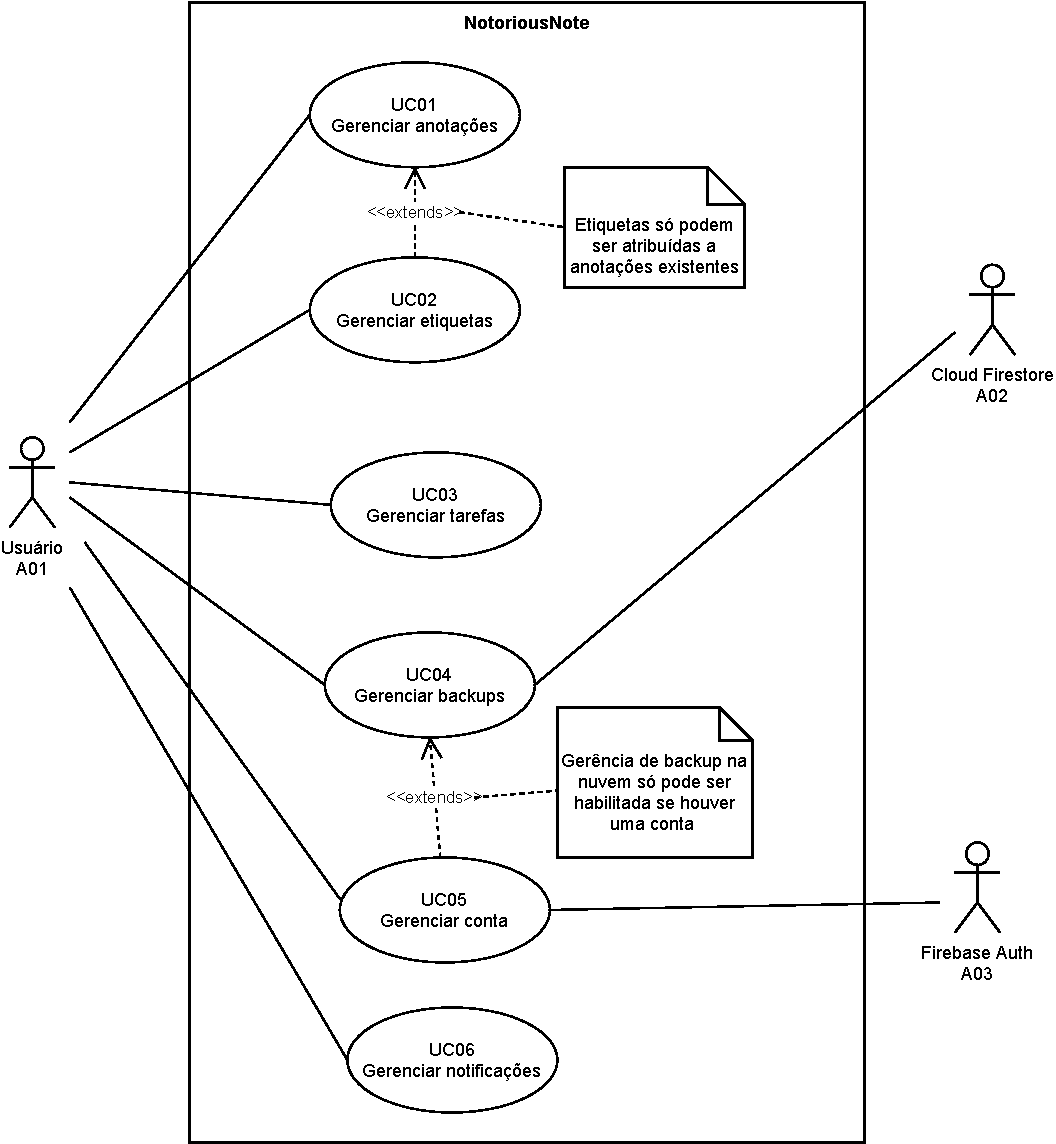
\includegraphics[keepaspectratio=true,width=0.8\textwidth]{notoriousnote-casos-de-uso.pdf}
    \caption{Diagrama de casos de uso do sistema}
    \label{fig:diagrama_casos_uso}
\end{figure}

\part{Especificação de casos de uso}

\chapter{UC01 - Gerenciar Anotações}

\section{Descrição} 
Caso de uso responsável por criar, ler, editar, excluir e arquivar anotações. O usuário interage com o sistema, que disponibiliza as possibilidades de gerência de anotações mencionadas previamente, e uma interface a edição e criação da anotação. Há a possibilidade das anotações serem arquivadas e visualizadas em uma interface diferente para melhor organização das anotações não prioritárias para o usuário.

\section{Atores}
\begin{itemize}
    \item[\textbf{Usuário}] Interessado em organizar seus compromissos em forma de anotações em texto.
\end{itemize}

\section{Regras de negócio}
\IBGEtabfontsize
\begin{longtable}{@{}lp{0.25\textwidth}p{0.6\textwidth}@{}}
\caption{Regras de negócio}
\label{tab:regras_de_negocio} \\
\toprule
\textbf{Id.} & \textbf{Nome} & \textbf{Descrição} \\ \midrule
RN01 & Validação de anotação & A anotação será considerada válida se houver conteúdo nos campos de título ou conteúdo. Isto é, anotações com um dos dois campos nulo ou vazio são válidas, e anotações com ambos os campos vazios são inválidas \phantomsection \label{uc01:rn01_validacao_anotacao} \\ \midrule
RN02 & Anotações arquivadas & Uma anotação é considerada arquivada se o conteúdo no campo numérico de arquivamento for configurado diferente de zero \phantomsection \label{uc01:rn02_flag_arquivar} \\ \bottomrule
\end{longtable}

\section{Fluxo básico de eventos}

\begin{enumerate}
    \item O usuário inicia aplicação
    \item O sistema carrega as anotações existentes \label{uc01:fluxo_base:carregar_anotacoes}
    \item Se houver anotações disponíveis será iniciado o fluxo alternativo de visualizar anotação (\ref{uc01:fluxo_alternativo:ler_anotacao_nao_arquivada})
    \item Se o usuário desejar visualizar as anotações arquivadas será iniciado o fluxo alternativo de ler anotação arquivada (\ref{uc01:fluxo_alternativo:ler_anotacao_arquivada})
    \item Se o usuário desejar criar uma anotação será iniciado o fluxo alternativo de criar anotação (\ref{uc01:fluxo_alternativo:criar_anotacao}).
    \item Se o usuário desejar apagar uma anotação será iniciado o fluxo alternativo de apagar anotação (\ref{uc01:fluxo_alternativo:apagar_anotacao_nao_arquivada})
    \item Se o usuário desejar editar uma anotação será iniciado o fluxo alternativo de editar anotação (\ref{uc01:fluxo_alternativo:editar_anotacao_nao_arquivada})
    \item O fluxo básico se encerra.
    
\end{enumerate}

\section{Fluxos alternativos}

% Área de funcionalidade
\subsection{Visualização de anotações}
% subfluxo
\subsubsection{Visualizar anotações} \label{uc01:fluxo_alternativo:ler_anotacao_nao_arquivada}
\begin{enumerate}   
    \item Todas as anotações não arquivadas são disponibilizadas para o usuário.
    \item O sistema disponibiliza título, o conteúdo e as etiquetas de cada uma das anotações.
    \item Encerra o fluxo alternativo e retorna para o fluxo básico no passo \ref{uc01:fluxo_base:carregar_anotacoes}.
\end{enumerate}

\subsubsection{Visualizar anotações arquivadas} \label{uc01:fluxo_alternativo:ler_anotacao_arquivada}
\begin{enumerate}
    \item Todas as anotações arquivadas (\hyperref[uc01:rn02_flag_arquivar]{RN02}) são disponibilizadas para o usuário.
    \item Caso o usuário deseje editar a anotação será seguido o fluxo de edição \ref{uc01:fluxo_alternativo:editar_anotacao_arquivada}
    \item Caso o usuário deseje apagar a anotação será seguido o fluxo alternativo de apagar anotação \ref{uc01:fluxo_alternativo:apagar_anotacao_arquivada}
    \item Caso o usuário deseje visualizar as anotações não arquivadas o fluxo alternativo encerra e retorna para o fluxo básico no passo \ref{uc01:fluxo_base:carregar_anotacoes}.
\end{enumerate}

% Área de funcionalidade
\subsection{Criação de anotações}
% subfluxo
\subsubsection{Criar anotação} \label{uc01:fluxo_alternativo:criar_anotacao}
\begin{enumerate}
    \item O sistema disponibiliza uma interface para criação da anotação
    \item O sistema carrega as etiquetas existentes
    \item O sistema disponibiliza edição do título, conteúdo, etiquetas e estado de arquivamento da anotação
    \item O usuário modifica título, conteúdo, etiquetas ou estado de arquivamento da anotação \label{uc01:fluxo_alternativo:criar_anotacao:pode_escrever}
    \item O usuário pode modificar o estado de arquivamento da anotação
    \item O usuário pode selecionar uma das etiquetas disponíveis para atribuí-la à anotação
    \item Caso o usuário cancele a operação de criação ele retornará para o fluxo básico no passo \ref{uc01:fluxo_base:carregar_anotacoes}.
    \item Caso o usuário selecione a opção de salvar a anotação ela deve obedecer às \hyperref[uc01:rn01_validacao_anotacao]{RN01} e \hyperref[uc01:rn02_flag_arquivar]{RN02}. Caso não obedeça, o caso vai para o fluxo excepcional \ref{uc01:fluxo_excepcional:criacao_invalida}.
    \item A anotação é criada com o título, conteúdo e etiquetas selecionadas pelo usuário
    \item Encerra o fluxo alternativo e retorna para o fluxo básico no passo \ref{uc01:fluxo_base:carregar_anotacoes}.
\end{enumerate}

% Área de funcionalidade
\subsection{Edição de anotações}
% subfluxo
\subsubsection{Editar anotação não arquivada} \label{uc01:fluxo_alternativo:editar_anotacao_nao_arquivada}
\begin{enumerate}
    \item O sistema disponibiliza uma interface para edição da anotação
    \item O sistema carrega título, conteúdo, etiquetas e estado de arquivamento da anotação a ser editada
    \item O sistema carrega as etiquetas existentes
    \item O sistema disponibiliza edição do título, conteúdo, etiquetas e estado de arquivamento da anotação
    \item O usuário modifica título, conteúdo, etiquetas ou estado de arquivamento da anotação \label{uc01:fluxo_alternativo:editar_anotacao_nao_arquivada:pode_escrever}
    \item O usuário pode modificar o estado de arquivamento da anotação
    \item O usuário pode selecionar uma das etiquetas disponíveis para atribuí-la à anotação
    \item Caso o usuário cancele a operação de criação ele retornará para o fluxo básico no passo \ref{uc01:fluxo_base:carregar_anotacoes}.
    \item Caso o usuário selecione a opção de salvar a anotação ela deve obedecer às \hyperref[uc01:rn01_validacao_anotacao]{RN01} e \hyperref[uc01:rn02_flag_arquivar]{RN02}. Caso não obedeça, o caso vai para o fluxo excepcional \ref{uc01:fluxo_excepcional:edicao_nao_arquivada_invalida}.
    \item A anotação é salva com o título, conteúdo e etiquetas selecionadas pelo usuário
    \item Encerra o fluxo alternativo e retorna para o fluxo básico no passo \ref{uc01:fluxo_base:carregar_anotacoes}.
\end{enumerate}

\subsubsection{Editar anotação arquivada} \label{uc01:fluxo_alternativo:editar_anotacao_arquivada}
\begin{enumerate}
    \item O sistema disponibiliza uma interface para edição da anotação
    \item O sistema carrega título, conteúdo, etiquetas e estado de arquivamento da anotação a ser editada
    \item O sistema carrega as etiquetas existentes
    \item O sistema disponibiliza edição do título, conteúdo, etiquetas e estado de arquivamento da anotação
    \item O usuário modifica título, conteúdo, etiquetas ou estado de arquivamento da anotação \label{uc01:fluxo_alternativo:editar_anotacao_arquivada:pode_escrever}
    \item O usuário pode modificar o estado de arquivamento da anotação
    \item O usuário pode selecionar uma das etiquetas disponíveis para atribuí-la à anotação
    \item Caso o usuário cancele a operação de criação ele retornará para o fluxo alternativo \ref{uc01:fluxo_alternativo:ler_anotacao_arquivada}.
    \item Caso o usuário selecione a opção de salvar a anotação ela deve obedecer às \hyperref[uc01:rn01_validacao_anotacao]{RN01} e \hyperref[uc01:rn02_flag_arquivar]{RN02}. Caso não obedeça, o caso vai para o fluxo excepcional \ref{uc01:fluxo_excepcional:edicao_arquivada_invalida}.
    \item A anotação é salva com o título, conteúdo e etiquetas selecionadas pelo usuário
    \item Encerra o fluxo alternativo e retorna para o fluxo básico no passo \ref{uc01:fluxo_base:carregar_anotacoes}.
\end{enumerate}

% Área de funcionalidade
\subsection{Apagar anotações}
% subfluxo
\subsubsection{Apagar anotação não arquivada} \label{uc01:fluxo_alternativo:apagar_anotacao_nao_arquivada}
\begin{enumerate}
    \item O sistema questiona o usuário se ele realmente deseja realizar essa operação
    \item Se o usuário confirmar o desejo, a anotação é excluída
    \item O fluxo se encerra e retorna ao fluxo básico no passo \ref{uc01:fluxo_base:carregar_anotacoes}
\end{enumerate}

\subsubsection{Apagar anotação arquivada} \label{uc01:fluxo_alternativo:apagar_anotacao_arquivada}
\begin{enumerate}
    \item O sistema questiona o usuário se ele realmente deseja realizar essa operação
    \item Se o usuário confirmar o desejo, a anotação é excluída
    \item O fluxo se encerra e retorna ao fluxo alternativo \ref{uc01:fluxo_alternativo:ler_anotacao_arquivada}
\end{enumerate}

\section{Fluxos excepcionais}

\subsection{Tentativa de salvar anotação inválida na criação} \label{uc01:fluxo_excepcional:criacao_invalida}
\begin{enumerate}
    \item O usuário deve ser informado da regra de negócio violada
    \item Caso retorna ao fluxo alternativo \ref{uc01:fluxo_alternativo:criar_anotacao} no passo \ref{uc01:fluxo_alternativo:criar_anotacao:pode_escrever}.
\end{enumerate}

\subsection{Tentativa de salvar anotação inválida na edição de anotação não arquivada} \label{uc01:fluxo_excepcional:edicao_nao_arquivada_invalida}
\begin{enumerate}
    \item O usuário deve ser informado da regra de negócio violada
    \item Caso retorna ao fluxo alternativo \ref{uc01:fluxo_alternativo:editar_anotacao_nao_arquivada} no passo \ref{uc01:fluxo_alternativo:editar_anotacao_nao_arquivada:pode_escrever}.
\end{enumerate}

\subsection{Tentativa de salvar anotação inválida na edição de anotação arquivada} \label{uc01:fluxo_excepcional:edicao_arquivada_invalida}
\begin{enumerate}
    \item O usuário deve ser informado da regra de negócio violada
    \item Caso retorna ao fluxo alternativo \ref{uc01:fluxo_alternativo:editar_anotacao_arquivada} no passo \ref{uc01:fluxo_alternativo:editar_anotacao_nao_arquivada:pode_escrever}.
\end{enumerate}

% \section{Subfluxos}
% Nenhum especificado

% \section{Cenários Chave}

% \section{Condições prévias}

\section{Condições posteriores}
\begin{enumerate}
    \item Após \ref{uc01:fluxo_alternativo:criar_anotacao} há a criação de anotações
    \item Após \ref{uc01:fluxo_alternativo:editar_anotacao_arquivada} e \ref{uc01:fluxo_alternativo:editar_anotacao_nao_arquivada} há a modificação das anotações existentes
    \item Após \ref{uc01:fluxo_alternativo:apagar_anotacao_arquivada} e \ref{uc01:fluxo_alternativo:apagar_anotacao_nao_arquivada} há o apagamento de anotações existentes
\end{enumerate}

\section{Pontos de extensão}
Os fluxos alternativos relativos à criação \ref{uc01:fluxo_alternativo:criar_anotacao} e a edição \ref{uc01:fluxo_alternativo:editar_anotacao_nao_arquivada} e \ref{uc01:fluxo_alternativo:editar_anotacao_arquivada} interagem com a leitura das etiquetas existentes e com a atribuição de etiquetas.

% \section{Requisitos especiais}

% \section{Informações adicionais}

% \chapter{Lições Aprendidas}
\chapter{Lições Aprendidas}
% [Liste as lições aprendidas na retrospectiva, com ênfase especial nas ações a serem tomadas para melhorar, por exemplo: o ambiente de desenvolvimento, o processo ou a colaboração da equipe.]
A equipe iniciou o desenvolvimento através de uma abordagem ágil da Engenharia de Requisitos. A troca da perspectiva de ágil para tradicional ajudou os componentes a trabalharem mapeando os problemas identificados anteriormente em necessidades, organizar estas em requisitos funcionais e agrupar esses requisitos em casos de uso.

No início da unidade 5 houve uma confusão sobre como se especificaria um caso de uso. Após conversas com o Professor Orientador, ficou evidente que não havia a necessidade de se seguir todos os pontos do \textit{template} apresentado como exemplo, o que simplificou a especificação.

% \begin{itemize}
% \section{Gerenciamento de atividades}
% \item a
% \item b
% \item c
% \section{Priorização de requisitos}
% \item a
% \item b
% \item c
% \section{Priorização de requisitos}
% \item a
% \item b
% \item c
% \end{itemize}

% ----------------------------------------------------------
% Capitulo com exemplos de comandos inseridos de arquivo externo
% ----------------------------------------------------------

% ---
% Este capítulo, utilizado por diferentes exemplos do abnTeX2, ilustra o uso de
% comandos do abnTeX2 e de LaTeX.
% ---

% \include{abntex2-modelo-include-comandos}

% ----------------------------------------------------------
% Parte de resultados
% ----------------------------------------------------------
% \part{Resultados}

% ---
% Capitulo de revisão de literatura
% ---
% \chapter{Lorem ipsum dolor sit amet}

% ---
% \section{Aliquam vestibulum fringilla lorem}
% ---

% \lipsum[1]

% \lipsum[2-3]

% ---
% Finaliza a parte no bookmark do PDF
% para que se inicie o bookmark na raiz
% e adiciona espaço de parte no Sumário
% ---
\phantompart

% ---
% Conclusão
% ---
% \chapter{Conclusão}
% ---

% \lipsum[31-33]

% ----------------------------------------------------------
% ELEMENTOS PÓS-TEXTUAIS
% ----------------------------------------------------------
\postextual

% ----------------------------------------------------------
% Referências bibliográficas
% ----------------------------------------------------------
%[Listar as referências utilizadas neste documento]
\bibliography{referencias_visao.bib}

% ----------------------------------------------------------
% Glossário
% ----------------------------------------------------------
%
% Consulte o manual da classe abntex2 para orientações sobre o glossário.
%
%\glossary

% ----------------------------------------------------------
% Apêndices
% ----------------------------------------------------------

% ---
% Inicia os apêndices
% ---
% \begin{apendicesenv}

% Imprime uma página indicando o início dos apêndices
% \partapendices

% ----------------------------------------------------------
% \chapter{Quisque libero justo}
% ----------------------------------------------------------

% \lipsum[50]

% ----------------------------------------------------------
% \chapter{Nullam elementum urna vel imperdiet sodales elit ipsum pharetra ligula
% ac pretium ante justo a nulla curabitur tristique arcu eu metus}
% ----------------------------------------------------------
% \lipsum[55-57]

% \end{apendicesenv}
% ---


% ----------------------------------------------------------
% Anexos
% ----------------------------------------------------------

% ---
% Inicia os anexos
% ---
% \begin{anexosenv}

% Imprime uma página indicando o início dos anexos
% \partanexos

% ---
% \chapter{Morbi ultrices rutrum lorem.}
% ---
% \lipsum[30]

% ---
% \chapter{Cras non urna sed feugiat cum sociis natoque penatibus et magnis dis
% parturient montes nascetur ridiculus mus}
% ---

% \lipsum[31]

% ---
% \chapter{Fusce facilisis lacinia dui}
% ---

% \lipsum[32]

% \end{anexosenv}

%---------------------------------------------------------------------
% INDICE REMISSIVO
%---------------------------------------------------------------------

\phantompart

\printindex

%---------------------------------------------------------------------
% Formulário de Identificação (opcional)
%---------------------------------------------------------------------
% \chapter*[Formulário de Identificação]{Formulário de Identificação}
% \addcontentsline{toc}{chapter}{Exemplo de Formulário de Identificação}
% \label{formulado-identificacao}

% Exemplo de Formulário de Identificação, compatível com o Anexo A (informativo)
% da ABNT NBR 10719:2015. Este formulário não é um anexo. Conforme definido na
% norma, ele é o último elemento pós-textual e opcional do relatório.

% \bigskip

% \begin{tabular}{|p{9cm}|p{5cm}|}
% \hline
% \multicolumn{2}{|c|}{\textbf{\large Dados do Relatório Técnico e/ou científico}}\\
% \hline
% \multirow{4}{10cm}[24pt]{Título e subtítulo}& Classificação de segurança\\
%                   & \\
%                   \cline{2-2}
%                   & No.\\
%                   & \\

% \hline
% Tipo de relatório & Data\\
% \hline
% Título do projeto/programa/plano & No.\\
% \hline
% \multicolumn{2}{|l|}{Autor(es)} \\
% \hline
% \multicolumn{2}{|l|}{Instituição executora e endereço completo} \\
% \hline
% \multicolumn{2}{|l|}{Instituição patrocinadora e endereço completo} \\
% \hline
% \multicolumn{2}{|l|}{Resumo}\\[3cm]
% \hline
% \multicolumn{2}{|l|}{Palavras-chave/descritores}\\
% \hline
% \multicolumn{2}{|l|}{
% Edição \hfill No. de páginas \hfill No. do volume \hfill Nº de classificação \phantom{XXXX}} \\
% \hline
% \multicolumn{2}{|l|}{
% ISSN \hfill \hfill Tiragem \hfill Preço \phantom{XXXXXXXX}} \\
% \hline
% \multicolumn{2}{|l|}{Distribuidor} \\
% \hline
% \multicolumn{2}{|l|}{Observações/notas}\\[3cm]
% \hline
% \end{tabular}

\end{document}